% Options for packages loaded elsewhere
\PassOptionsToPackage{unicode}{hyperref}
\PassOptionsToPackage{hyphens}{url}
%
\documentclass[
]{article}
\usepackage{amsmath,amssymb}
\usepackage{iftex}
\ifPDFTeX
  \usepackage[T1]{fontenc}
  \usepackage[utf8]{inputenc}
  \usepackage{textcomp} % provide euro and other symbols
\else % if luatex or xetex
  \usepackage{unicode-math} % this also loads fontspec
  \defaultfontfeatures{Scale=MatchLowercase}
  \defaultfontfeatures[\rmfamily]{Ligatures=TeX,Scale=1}
\fi
\usepackage{lmodern}
\ifPDFTeX\else
  % xetex/luatex font selection
\fi
% Use upquote if available, for straight quotes in verbatim environments
\IfFileExists{upquote.sty}{\usepackage{upquote}}{}
\IfFileExists{microtype.sty}{% use microtype if available
  \usepackage[]{microtype}
  \UseMicrotypeSet[protrusion]{basicmath} % disable protrusion for tt fonts
}{}
\makeatletter
\@ifundefined{KOMAClassName}{% if non-KOMA class
  \IfFileExists{parskip.sty}{%
    \usepackage{parskip}
  }{% else
    \setlength{\parindent}{0pt}
    \setlength{\parskip}{6pt plus 2pt minus 1pt}}
}{% if KOMA class
  \KOMAoptions{parskip=half}}
\makeatother
\usepackage{xcolor}
\usepackage[margin=1in]{geometry}
\usepackage{graphicx}
\makeatletter
\def\maxwidth{\ifdim\Gin@nat@width>\linewidth\linewidth\else\Gin@nat@width\fi}
\def\maxheight{\ifdim\Gin@nat@height>\textheight\textheight\else\Gin@nat@height\fi}
\makeatother
% Scale images if necessary, so that they will not overflow the page
% margins by default, and it is still possible to overwrite the defaults
% using explicit options in \includegraphics[width, height, ...]{}
\setkeys{Gin}{width=\maxwidth,height=\maxheight,keepaspectratio}
% Set default figure placement to htbp
\makeatletter
\def\fps@figure{htbp}
\makeatother
\setlength{\emergencystretch}{3em} % prevent overfull lines
\providecommand{\tightlist}{%
  \setlength{\itemsep}{0pt}\setlength{\parskip}{0pt}}
\setcounter{secnumdepth}{-\maxdimen} % remove section numbering
\ifLuaTeX
  \usepackage{selnolig}  % disable illegal ligatures
\fi
\IfFileExists{bookmark.sty}{\usepackage{bookmark}}{\usepackage{hyperref}}
\IfFileExists{xurl.sty}{\usepackage{xurl}}{} % add URL line breaks if available
\urlstyle{same}
\hypersetup{
  pdftitle={TimeMixedEffectsModel},
  pdfauthor={-``Aissata Bah'' -``Brice Laurent'' -``Linh Vu''},
  hidelinks,
  pdfcreator={LaTeX via pandoc}}

\title{TimeMixedEffectsModel}
\author{-``Aissata Bah'' -``Brice Laurent'' -``Linh Vu''}
\date{2023-12-07}

\begin{document}
\maketitle

\hypertarget{theory-behind-using-linear-mixed-effects-model-for-time}{%
\section{Theory Behind Using Linear Mixed Effects Model for
Time}\label{theory-behind-using-linear-mixed-effects-model-for-time}}

\[HDI_{year,region} = \alpha_{region}+\beta_{region}X_{year,country,region}+\varepsilon_{country,region}\]
where \(\alpha_{region}\sim N(\mu_{\alpha},\sigma_{\alpha}^2)\) and
\(\beta_{region}\sim N(\mu_{\beta},\sigma_{\beta}^2)\)

This equation is assuming no correlation between the random effects.
However, from the following plot, we can see that the average HDI of all
the regions seem to follow a similar trajectory over time and,
therefore, we would expect the random effects to be correlated between
regions. Because of this, we will allow for correlation between random
effects, for which there is a closed form solution.

\begin{verbatim}
## `summarise()` has grouped output by 'region'. You can override using the
## `.groups` argument.
\end{verbatim}

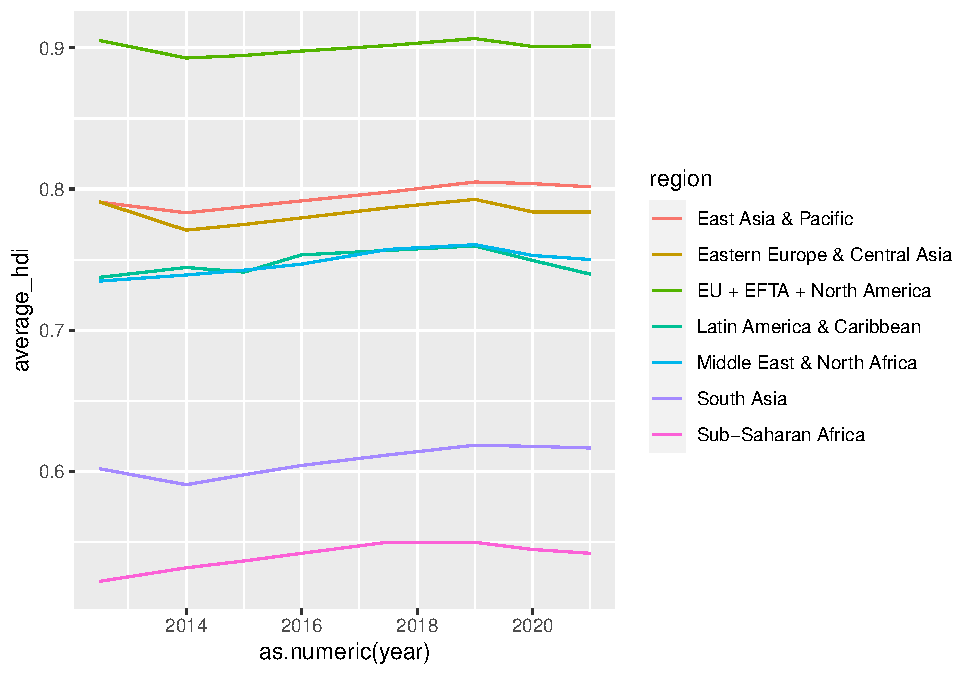
\includegraphics{TimeMixedEffectsModel_files/figure-latex/unnamed-chunk-2-1.pdf}

\begin{verbatim}
## Warning in checkConv(attr(opt, "derivs"), opt$par, ctrl = control$checkConv, :
## Model failed to converge with max|grad| = 0.0038418 (tol = 0.002, component 1)
\end{verbatim}

\begin{verbatim}
## Warning: Model failed to converge with 1 negative eigenvalue: -2.8e+00
\end{verbatim}

\begin{verbatim}
##                 Estimate  Std. Error       df    t value     Pr(>|t|)
## (Intercept)  0.702555461 0.051747797 5.868732 13.5765288 1.179044e-05
## x1.6         0.002427165 0.012521861 6.047902  0.1938342 8.526523e-01
## x3.2         0.001812547 0.004586301 7.969709  0.3952089 7.030559e-01
## x5.1        -0.005945864 0.010641112 5.504172 -0.5587634 5.982981e-01
## x6.4        -0.010689390 0.009729157 4.673279 -1.0986964 3.252537e-01
## x7.3         0.015843354 0.014052895 5.982112  1.1274086 3.027497e-01
\end{verbatim}

Degrees of Freedom=Total number of observations−Number of fixed
effects−Number of estimated variance components

Bonferroni Correction: \(\alpha\)=0.05/6=0.00833

\begin{verbatim}
## refitting model(s) with ML (instead of REML)
\end{verbatim}

\begin{verbatim}
## Warning in optwrap(optimizer, devfun, x@theta, lower = x@lower, calc.derivs =
## TRUE, : convergence code 1 from bobyqa: bobyqa -- maximum number of function
## evaluations exceeded
\end{verbatim}

\begin{verbatim}
## Data: selected_columns
## Models:
## time_mixed_effects_noRegion: hdi ~ x1.6 + x3.2 + x5.1 + x6.4 + x7.3 + (1 + years_from_2000 || country)
## time_mixed_effects: hdi ~ x1.6 + x3.2 + x5.1 + x6.4 + x7.3 + (1 + x1.6 + x3.2 + x5.1 + x6.4 + x7.3 | region) + (1 + years_from_2000 || country)
##                             npar     AIC     BIC logLik deviance  Chisq Df
## time_mixed_effects_noRegion    9 -5315.0 -5271.7 2666.5  -5333.0          
## time_mixed_effects            30 -5412.7 -5268.2 2736.3  -5472.7 139.66 21
##                             Pr(>Chisq)    
## time_mixed_effects_noRegion               
## time_mixed_effects           < 2.2e-16 ***
## ---
## Signif. codes:  0 '***' 0.001 '**' 0.01 '*' 0.05 '.' 0.1 ' ' 1
\end{verbatim}

\begin{verbatim}
## Warning in checkConv(attr(opt, "derivs"), opt$par, ctrl = control$checkConv, :
## Model failed to converge with max|grad| = 0.00405253 (tol = 0.002, component 1)
\end{verbatim}

\begin{verbatim}
## refitting model(s) with ML (instead of REML)
\end{verbatim}

\begin{verbatim}
## Warning in optwrap(optimizer, devfun, x@theta, lower = x@lower, calc.derivs =
## TRUE, : convergence code 1 from bobyqa: bobyqa -- maximum number of function
## evaluations exceeded
\end{verbatim}

\begin{verbatim}
## Data: selected_columns
## Models:
## time_mixed_effects_noYear: hdi ~ x1.6 + x3.2 + x5.1 + x6.4 + x7.3 + (1 + x1.6 + x3.2 + x5.1 + x6.4 + x7.3 | region)
## time_mixed_effects: hdi ~ x1.6 + x3.2 + x5.1 + x6.4 + x7.3 + (1 + x1.6 + x3.2 + x5.1 + x6.4 + x7.3 | region) + (1 + years_from_2000 || country)
##                           npar     AIC     BIC logLik deviance  Chisq Df
## time_mixed_effects_noYear   28 -3045.2 -2910.4 1550.6  -3101.2          
## time_mixed_effects          30 -5412.7 -5268.2 2736.3  -5472.7 2371.4  2
##                           Pr(>Chisq)    
## time_mixed_effects_noYear               
## time_mixed_effects         < 2.2e-16 ***
## ---
## Signif. codes:  0 '***' 0.001 '**' 0.01 '*' 0.05 '.' 0.1 ' ' 1
\end{verbatim}

\includegraphics{TimeMixedEffectsModel_files/figure-latex/unnamed-chunk-6-1.pdf}
\includegraphics{TimeMixedEffectsModel_files/figure-latex/unnamed-chunk-6-2.pdf}

\includegraphics{TimeMixedEffectsModel_files/figure-latex/unnamed-chunk-7-1.pdf}

\end{document}
